%************************************************
%\chapter{Trends in CO$_2$ flux} % $\mathbb{ZNR}$
\chapter{Processes corresponding to multi-year trends in sea-air CO$_2$ flux}
%************************************************
\label{ch:trends}

%\section[Winds determine internal variability]{Winds determine internal variability of the Southern Ocean CO$_2$ flux}
%\section[Westerly winds and Southern Ocean CO$_2$ flux variability]{The role of westerly winds on Southern Ocean CO$_2$ flux variability}
\section{The role of westerly winds in Southern Ocean CO$_2$ flux variability}

%\paragraph{on area 50-60S as driver of Southern Ocean internal variability, correlation plots co2flux and wind trends} 
\cite{Thompson2000} and \cite{Hall2002} describe the \acf{SAM} as the most dominant mode for higher-latitude Southern Hemisphere variability. \citeauthor{Lovenduski2007} [{\color{RoyalBlue}2007}] explain the influence of the westerly winds on the Southern Ocean carbon sink. 

To further assess internal variability due to westerly winds in \acs{MPI}-\acs{ESM} this chapter discusses the effect of westerly winds on the thermal, physical and biological controls of the Southern Ocean carbon sink in \acs{HAMOCC}.\newline

I find a correlation on 8-year trends between \acs{SAM}, which describes the position and latitudinal shift of westerly winds, and the CO$_2$ flux in the area of largest decadal internal variability at 50-60$^\circ$S (\autoref{fig:scatter}). Although the CO$_2$ flux formula (\autoref{sec:HAMOCC}) also depends on the wind speed at 10m height, the driver of the changes in \autoref{fig:scatter} is not the piston velocity $k_w$, but in $\Delta \text{pCO}_2$ \citep{Lovenduski2015}. However, the magnitude of short-term variability on the timescale of days to hours depends highly on wind strength variability whereas the direction of CO$_2$ flux is independent of wind speed. This relationship reveals two distinct regimes of wind-driven CO$_2$ flux signals in this area: 

Intensified and southward-shifted winds, associated with an increasing trend in \acs{SAM}, lead to a positive CO$_2$ flux trend. This Southern Ocean carbon sink response has been suggested frequently for the observed and projected trend in \acs{SAM} \citep{LeQuere2007,Lovenduski2007,Lovenduski2008,Hauck2013,landschuetzer2015}. The related process responses corresponding to stronger winds are explained in \autoref{sec:trends_pos}.

In \acs{MPI-ESM} I also find the reverse case of weakening and northward-shifting westerly winds, associated with a negative trend in \acs{SAM}, which lead to a negative CO$_2$ flux or ocean uptake trend. The responses of processes corresponding to weaker winds are explained in \autoref{sec:trends_neg}. However, observations do not reveal a strong multi-year negative \acs{SAM} trend (\autoref{fig:evolution_SAM}). Likewise, westerly winds did not weaken but continued to increase during the negative CO$_2$ flux trend in the 2000s \citep{landschuetzer2015}. On the contrary, depending on the starting year of the trend period, the \acs{SAM} index slightly weakened in the early 2000s \citep{Marshall2003,Lovenduski2015}, and also \cite{DeVries2017} report a decline in upper-ocean overturning circulation which may be connected to strength and position of winds. \newline

The strong trends originate in strong changes of the position and strength of Southern hemisphere westerly winds and effect of those on ocean circulation. Though the parametrized eddies in \acs{MPI-ESM LE} might allow deeper mixing to sustain for multiple years and hence longer than the seasonal timescale at which the eddies would counteract those trends \citep{Thompson2011}. Only a variable definition of isopyncal thickness diffusion could parametrize the expected eddy response from high-resolution simulations \citep{Gent2011}. These enhanced eddy fluxes in a low-resolution model are discussed in \cite{Lovenduski2013}.


\begin{figure}[h!]
\centering
%		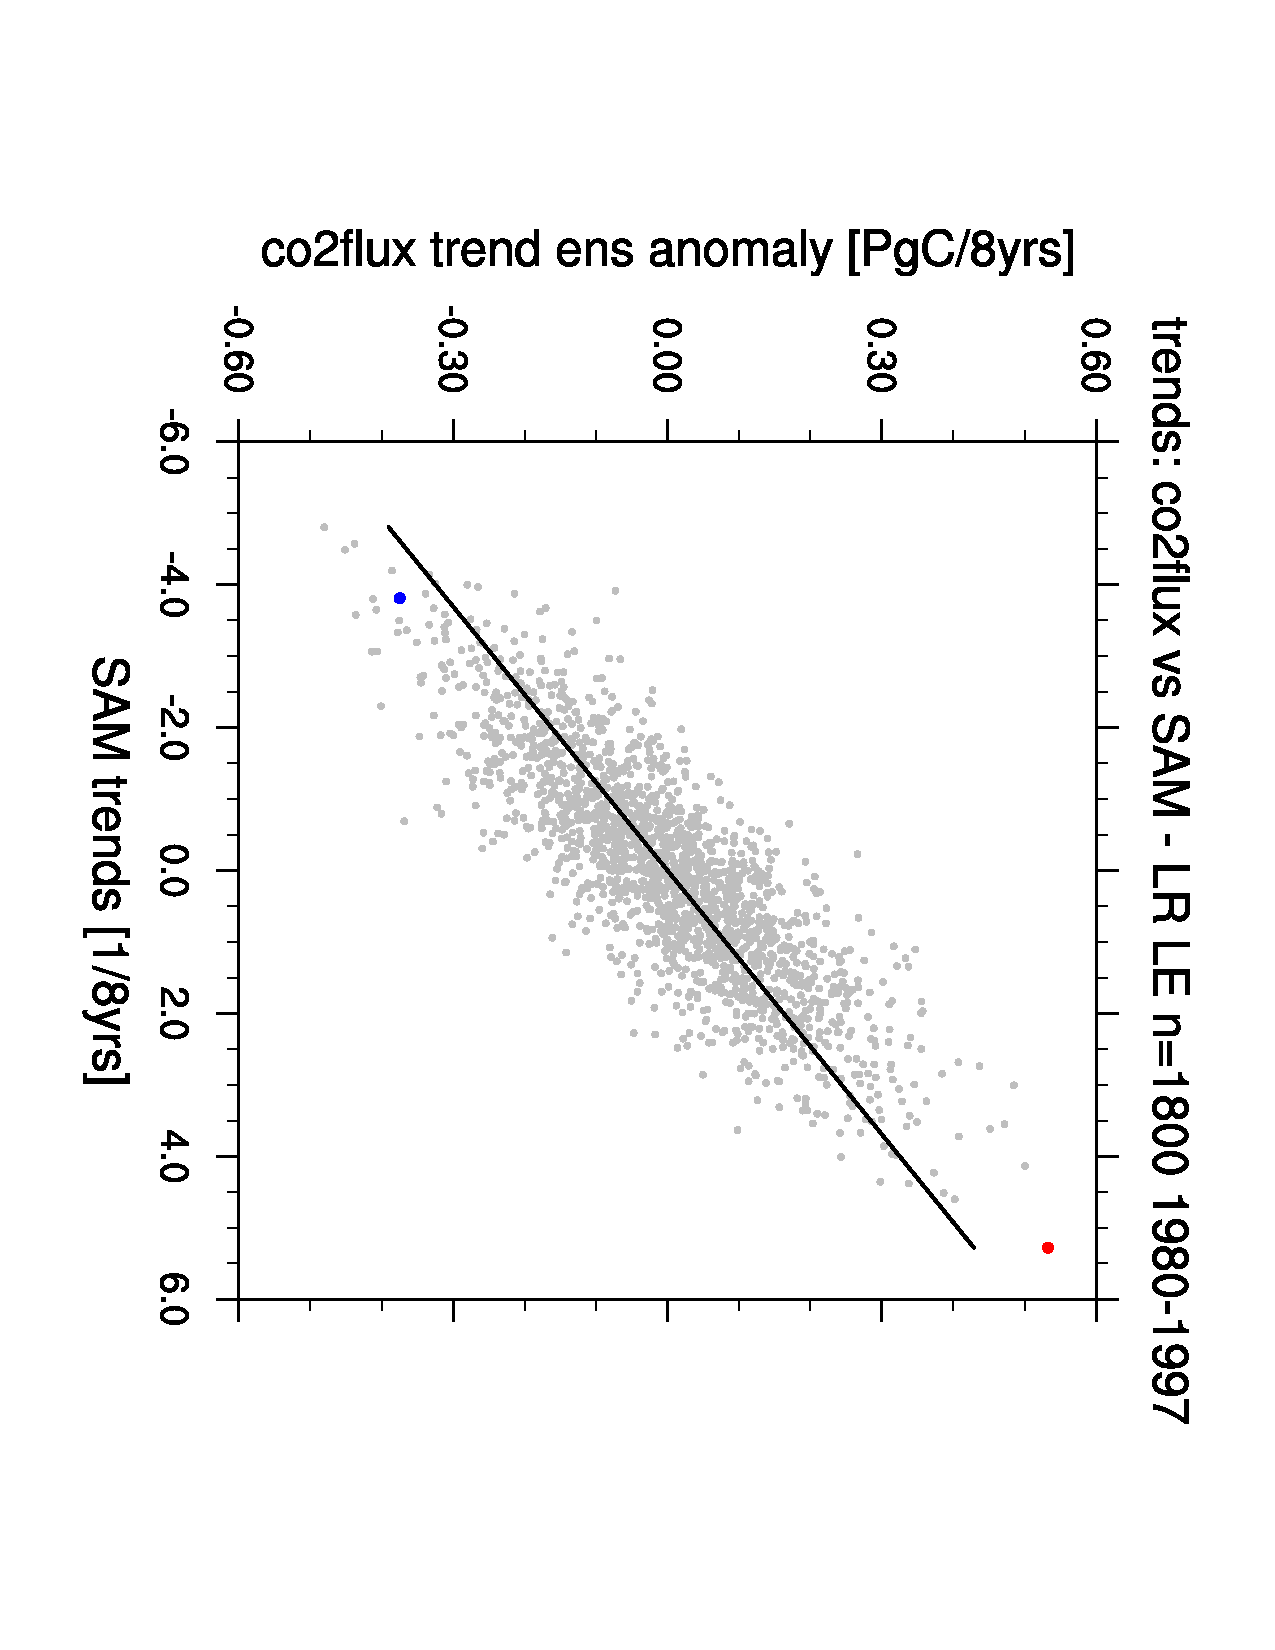
\includegraphics[scale=.5,page=1,angle=90,trim=1.3cm 2.3cm 2.3cm 3cm,clip]{Scatter_trends_bands_ensanom_co2flux_vs_SAM_n1800_1980_1997_trend8_50-59S}
		\captionsetup[subfigure]{labelformat=empty,justification=centering}
		\subfloat[Sea-air CO$_2$ vs. \acf{SAM}]{		
		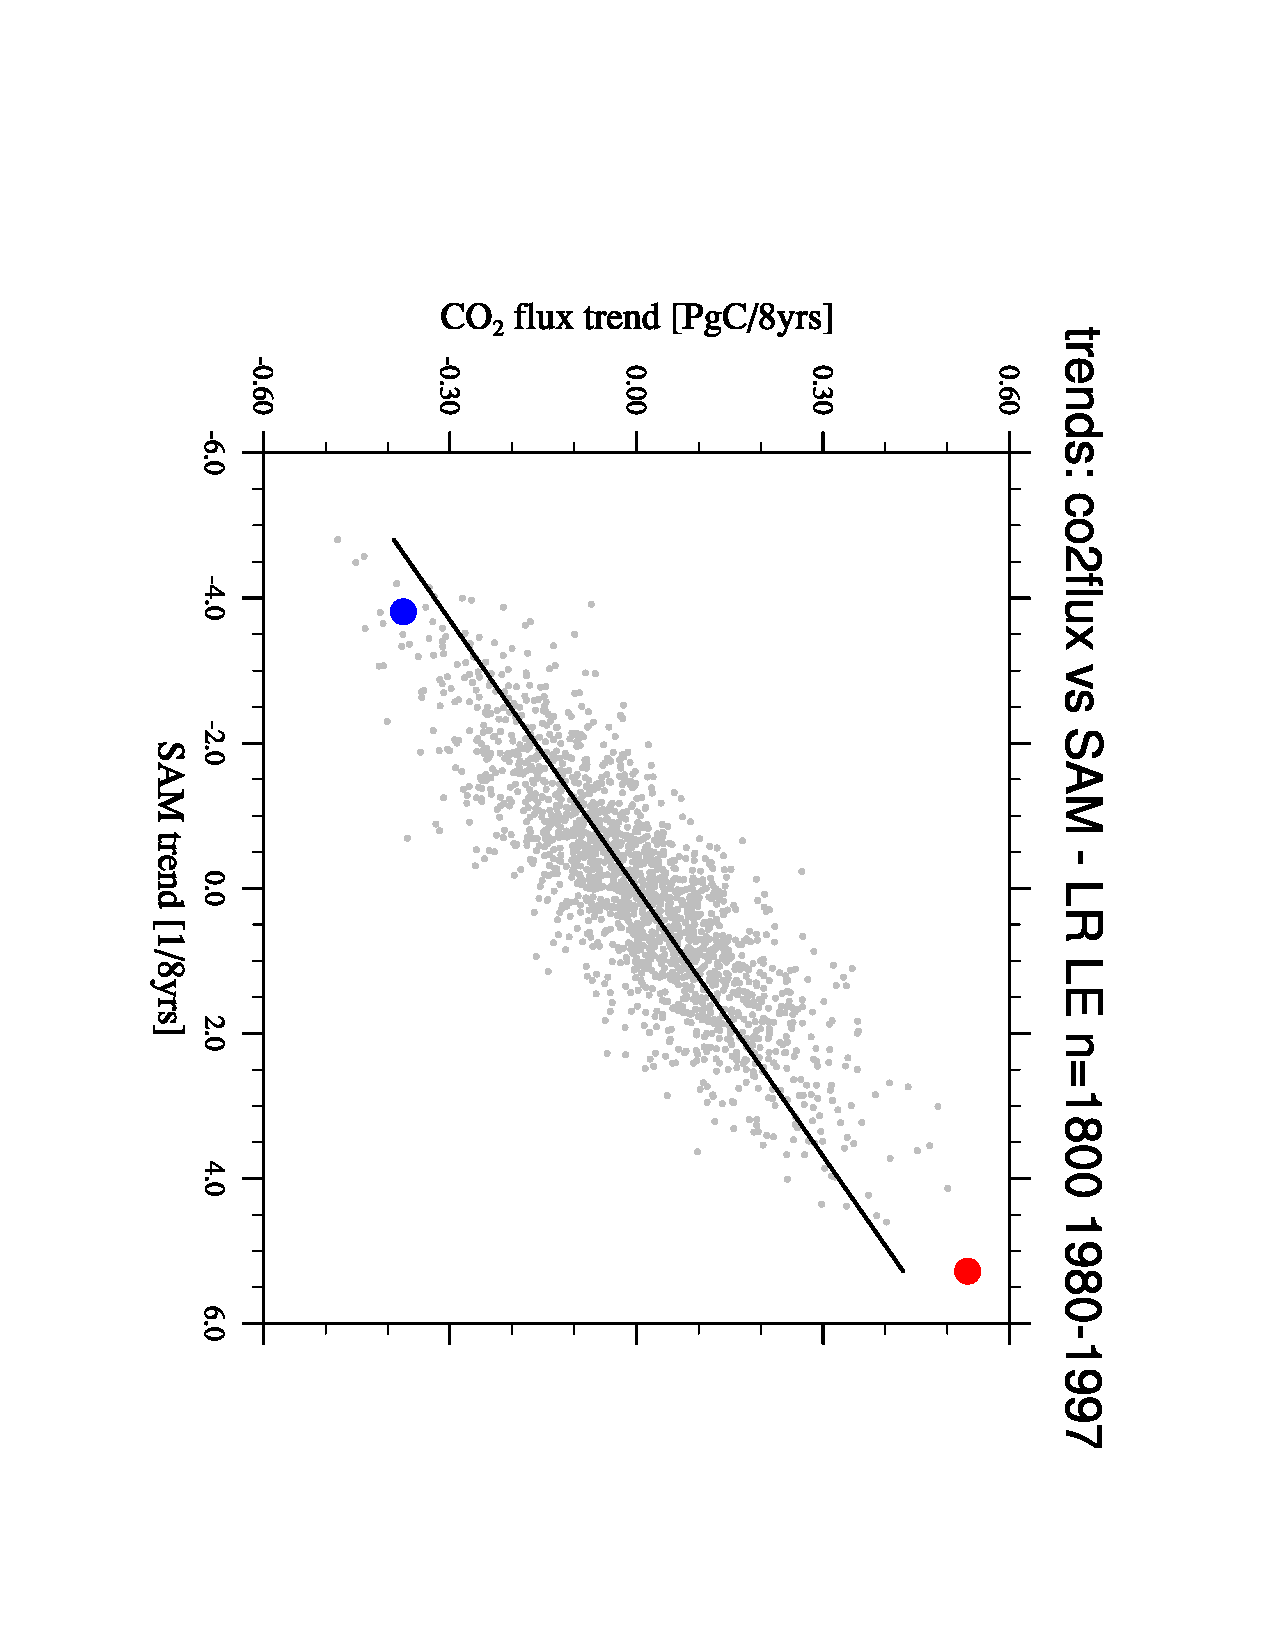
\includegraphics[scale=.6,page=1,angle=90,trim=1.3cm 2.3cm 3.8cm 4cm,clip]{EGU_new_SAM_Scatter_trends_bands_ensanom_co2flux_vs_SAM_n1800_1980_1997_trend8}}		
		%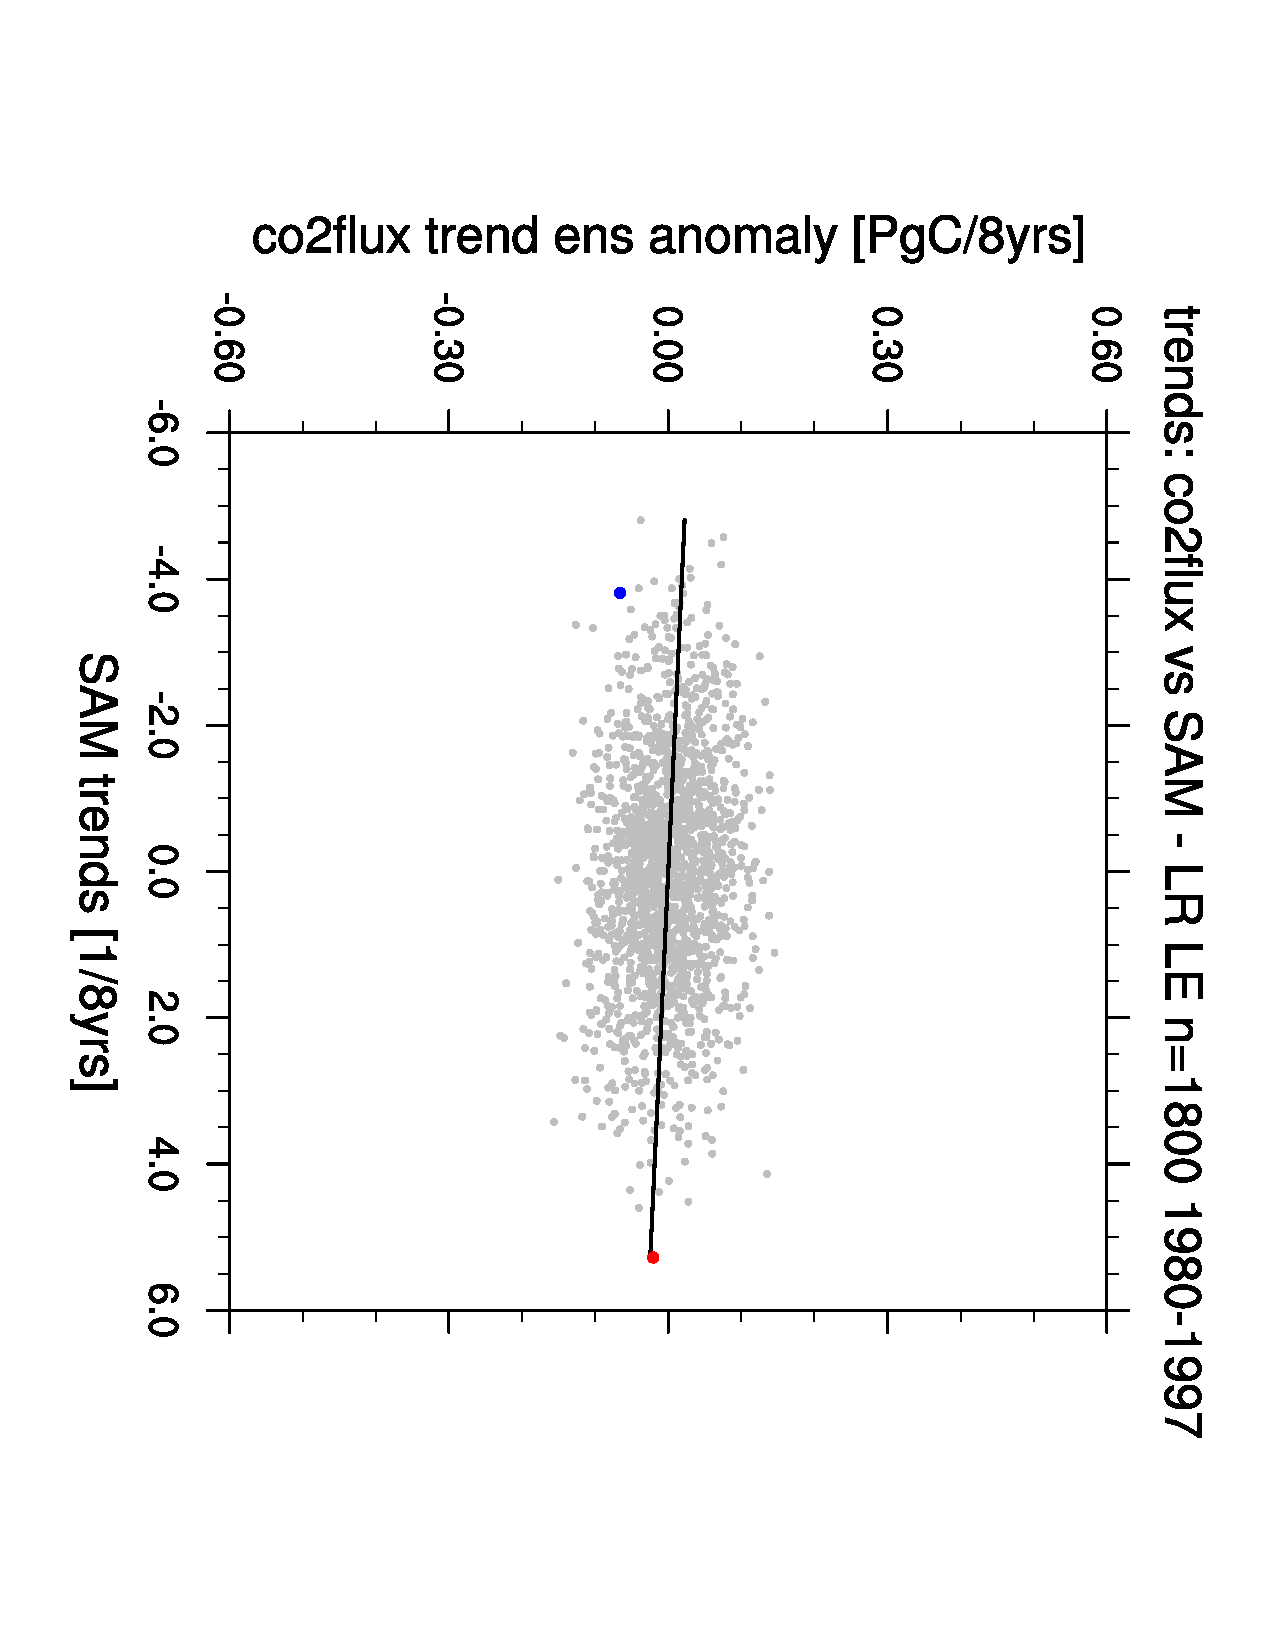
\includegraphics[scale=.38,page=1,angle=90,trim=1.3cm 2.3cm 2.3cm 3cm,clip]{Scatter_trends_bands_ensanom_co2flux_vs_SAM_n1800_1980_1997_trend8_40-49S}
		\vspace{-2mm}
		\caption{Linear trends in the \ac{SAM} as indicator of wind strength vs. sea-air CO$_2$ flux at 50-60$^\circ$S; each data point represents 8-year trends of a single realization normalized for the ensemble mean trend  between 1980 and 2004; the blue dot represents the most negative monotonic CO$_2$ flux trend; the red dot the positive monotonic CO$_2$ flux trend.}
		\label{fig:scatter}
\end{figure}

To qualitatively understand the mechanisms of the Southern Ocean carbon sink I analyze the drivers of CO$_2$ flux on a process level. This chapter covers qualitative CO$_2$ flux changes with respect to the thermal effect, physical circulation and biology. A quantitative analysis of the different drivers for different regions follows in \autoref{ch:pCO2separation}.

The analysis presented here involves 8-year trends for reasons stated in \autoref{sec:choicetrend} but the results of this chapter apply to various multi-year and decadal trends subject to internal variability (not shown).

The spatial trend patterns of different trend periods mostly appear zonally symmetric, therefore the analysis is not separated into the different Southern Ocean sectors, \eg in the Pacific, Indian or Atlantic sector. Also, the atmospheric circulation change in \acs{MPI-ESM} is too symmetric compared to observations \citep{Haumann2014}. Therefore, the description here is carried out in zonal latitudinal bands keeping the unsymmetrical Southern Ocean dynamics in mind \citep{Sallee2010,Talley2013}. Also due to the underestimated Antarctic sea-ice and open-ocean convection in the Ross and Weddell Sea, I restrict my analysis to the Southern Ocean north of 60$^\circ$S, but the decadal CO$_2$ flux trends have a weak signal south of 60$^\circ$S anyway. 



\clearpage

\section{Positive CO$_2$ flux trends}
\label{sec:trends_pos}

Strong positive CO$_2$ flux trends correlate with stronger westerly winds (\autoref{fig:scatter}) \citep{Lovenduski2007}. The difference $\Delta$pCO$_2$ between oceanic pCO$_{2,\text{ocean}}$ and atmospheric partial pressures pCO$_{2,\text{atm}}$ depicts a cleaner signal than CO$_2$ flux (\autoref{fig:pos-co2flux},\ref{fig:pos-dpco2}) and is independent of wind speed and solubility \citep{Lovenduski2015}. pCO$_{2,\text{ocean}}$ rises stronger than pCO$_{2,\text{atm}}$, so CO$_2$ must be driven by changes in the ocean dynamics (\autoref{fig:pos-dpco2}).
The strongest positive signal occurs in the upwelling at 50-60$^\circ$S, a weaker and more patchy signal occurs in the subduction areas north of 50$^\circ$S, whereas changes in most other areas of the Southern Ocean are insignificant (\autoref{fig:pos-dpco2}). 

Westerly winds decrease at 40-50$^\circ$S and increase at 50-60$^\circ$S, which results in a southward shift of westerlies (\autoref{fig:pos-slp}) represented by the positive trend in \acs{SAM} (\autoref{fig:evolution_SAM}). \newline


The response of the thermal effect, upper-ocean overturning circulation and biology are described in \autoref{sec:trends_pos_thermal}, \ref{sec:trends_pos_circulation} and \ref{sec:trends_pos_biology}, respectively.

\begin{figure}[bth]
        \myfloatalign
        \subfloat[CO$_2$ flux trend \text{[kgC m$^{-2}$yr$^{-1}$ /8yrs]}]
        {\label{fig:pos-co2flux}%
        \includegraphics[scale=1.55,trim=13.2cm 18.75cm 4.5cm 6.3cm,clip]{\memberpositive _positive_trend_8_obgc_overview_co2.pdf}} %\quad
        \subfloat[$\Delta$pCO$_2$ trend \text{[ppm/8yrs]}]
        {\label{fig:pos-dpco2}%
         \includegraphics[scale=1.55,trim=13.2cm 15.9cm 4.5cm 9.225cm,clip]{\memberpositive _positive_trend_8_obgc_overview_co2.pdf}} \\
         
         \subfloat[\ac{SLP} and wind trends \text{[hPa/8yrs]}]
        {\label{fig:pos-slp}%
        \includegraphics[scale=1.55,trim=13.2cm 10.2cm 4.5cm 14.9cm,clip]{\memberpositive _positive_trend_8_obgc_overview_co2.pdf}} %\quad
        \subfloat[\ac{SST} trend \text{[$^{\circ}$C/8yrs]}]
        {\label{fig:pos-sst}%
         \includegraphics[scale=1.55,trim=13.18cm 13.05cm 4.5cm 12.075cm,clip]{\memberpositive _positive_trend_8_obgc_overview_co2.pdf}} \\
        \caption{Linear trends during the most positive monotonic 8-year sea-air CO$_2$ flux trend: (a) sea-air CO$_2$ flux, (b) $\Delta$pCO$_2$, (c) \ac{SLP} and wind vectors overlain as arrows and (d) \acf{SST}; hatched areas indicate where trends are outside the 5\% significance level.} \label{fig:pos}
\end{figure}



\clearpage

\subsection{Changes in the thermal effect during positive CO$_2$ flux trends}
\label{sec:trends_pos_thermal}
The solubility of pCO$_{\text{2,ocean}}$ is primarily sensitive to \acf{SST}. Warmer oceans such as the tropical oceans own a lower solubility than cooler high-latitude oceans - a process referred to as the solubility pump of carbon \citep{VolkHoffert1985}. Likewise, CO$_2$-equilibrated waters outgas when warmed and take up CO$_2$ when cooled.

The difference between the partial pressure of CO$_2$ in the ocean (pCO$_{2,\text{ocean}}$) and the atmosphere (pCO$_{2,\text{atm}}$) is the main changing quantity in the CO$_2$ flux formula \citep{Lovenduski2015} (\autoref{eq:HAMOCC}). The separation by \citeauthor{Takahashi1993} [{\color{RoyalBlue}1993}, {\color{RoyalBlue}2002}] gives insights about the direct influence of \ac{SST} (\autoref{sec:takahashi}). The thermal pCO$_2$ trend is driven by changes in \acs{SST} (\autoref{fig:thermal_pos-a}), whereas the non-thermal $\Delta $pCO$_2$ trend approximates all other changes in pCO$_{2,\text{atm}}$, biology, alkalinity, assuming constant \acs{SST} (\autoref{fig:thermal_pos-b}). The thermal pCO$_2$ trend and non-thermal $\Delta$pCO$_2$ trend approximately add up to the trends in pCO$_2$ \citep{landschuetzer2015}. 
The thermal trend follows the \acs{SST} cooling trend (\autoref{fig:pos-sst}) south of 50$^\circ$S towards negative CO$_2$ flux trends, whereas the warming north of 50$^\circ$S favors outgassing. Increased Ekman transport causes this heat divergence in polar regions and a heat convergence at lower latitudes \citep{Hall2002} (\autoref{fig:UOOC_pos}). The non-thermal component strongly increases south of 50$^\circ$S, so overall the pCO$_{2,\text{ocean}}$ increases faster than pCO$_{2,\text{atm}}$ leading to a positive sea-air CO$_2$ flux trend. %This reflects the enhanced outgassing from increased upwelling. 
The non-thermal and thermal trends combined nearly compensate north of 50$^\circ$S but at 50-60$^\circ$S the outgassing dominates (\autoref{fig:pos-dpco2}). The homogenous increase in atmospheric pCO$_{\text{2,atm}}$ accounts for a -12ppm/8yrs in $\Delta$pCO$_2$ (\autoref{fig:pos-dpco2}). %
These changes are stronger in the summer season, especially the non-thermal component because of the stronger summer \acs{SLP} trend (\autoref{fig:pos_summer}, \ref{fig:pos_winter}). 

\begin{figure}[bth]
        \myfloatalign
        \subfloat[pCO$_{\text{2,thermal}}$ trend \text{[ppm/8yrs]}]
        {\label{fig:thermal_pos-a}%
        \includegraphics[scale=1.55,trim=13.2cm 7.3cm 4.5cm 17.785cm,clip]{\memberpositive _positive_trend_8_obgc_overview_co2.pdf}} %\quad
        \subfloat[$\Delta$pCO$_{\text{2,non-thermal}}$ trend \text{[ppm/8yrs]}]
        {\label{fig:thermal_pos-b}%
         \includegraphics[scale=1.55,trim=13.2cm 4.5cm 4.4cm 20.65cm,clip]{\memberpositive _positive_trend_8_obgc_overview_co2.pdf}} \\
        \caption{Linear trends during the most positive monotonic 8-year sea-air CO$_2$ flux trend: (a) pCO$_{2,\text{thermal}}$ and (b) $\Delta$pCO$_{2,\text{non-thermal}}$; hatched areas indicate where trends are outside the 5\% significance level.} \label{fig:thermal_pos}
\end{figure}


\clearpage

\subsection{Changes in ocean circulation during positive CO$_2$ flux trends}
\label{sec:trends_pos_circulation}

Stronger westerly winds intensify the upper-ocean overturning circulation \citep{Lauderdale2013}. Therefore the circulation field advects more \acs{DIC} and alkalinity along its overturning pathway (\autoref{fig:UOOC_pos}). Intensified upwelling of super-saturated waters at 50-60$^\circ$S increase \acs{DIC} and alkalinity concentrations in the euphotic zone (\autoref{fig:ekman_pos-b}). As the pCO$_{\text{2,ocean}}$ sensitivity of \acs{DIC} is larger than for alkalinity, this likely enhances pCO$_{\text{2,ocean}}$, which leads to a positive CO$_2$ flux (for a detailed dicussion see \autoref{ch:pCO2separation}). The stronger winds also increase Ekman northward transport and advects \acs{DIC} and alkalinity further northward (\autoref{fig:ekman_pos-a}). Subduction rates of \ac{AAIW} and \ac{SAMW} formation increase north of 50$^\circ$S, so pCO$_{2,\text{atm}}$-equilibrated waters take additional anthropogenic carbon into the deeper ocean. The southward shift of westerly winds weakens the northern edge of Ekman transport at 30-40$^\circ$S. 

The changes in \ac{MLD} also contribute to the vertical transport of carbon. By deeper mixing in winter, more carbon-rich waters are included into the \acs{MLD}, which then serves as a larger super-saturated reservoir. \acs{MLD} deepens south of 50$^\circ$S and slightly shoals north of 45$^\circ$S, whereas open-ocean convection causes the unrealistic zonal \acs{MLD} averages below 300m south of 60$^\circ$S (\autoref{fig:UOOC_pos}) \citep{Sallee2013,Stoessel2015}. 



\begin{figure}[bth]
        \myfloatalign
        \subfloat[Ekman transport trend \text{[m$^2$ s$^{-1}$/8yrs]}]
        {\label{fig:ekman_pos-a}%
        \includegraphics[scale=1.5,trim=13.1cm 18.75cm 4.5cm 6.38cm,clip]{\memberpositive _positive_trend_8_ekman_overview.pdf}} %\quad
        \subfloat[Ekman pumping trend \text{[m s$^{-1}$/8yrs]}]
        {\label{fig:ekman_pos-b}%
         \includegraphics[scale=1.5,trim=13.25cm 15.9cm 4.1cm 9.2cm,clip]{\memberpositive _positive_trend_8_ekman_overview.pdf}} \\
        \caption{Linear trends during the most positive 8-year sea-air CO$_2$ flux trend: (a) Ekman transport and (b) Ekman pumping; hatched areas indicate where trends are outside the 5\% significance level.} \label{fig:ekman_pos}
\end{figure}


\begin{figure}[hbt]
	\centering
    \captionsetup[subfigure]{labelformat=empty,justification=centering}
	\subfloat[Carbon advection trends \text{[PgC/8yrs]}]{ 
	\includegraphics[scale=0.42,page=2,trim=.3cm 1.7cm 0cm 4.6cm,clip]{UOOC}}
	%\vspace{-5mm}
	\caption{Zonally averaged upper-ocean overturning circulation during the most positive 8-year sea-air CO$_2$ flux trend; black arrows show mean advective carbon transport, red arrows show advective carbon transport trends enforcing the upper-ocean overturning circulation; blue arrows show advective carbon transport trends weakening the upper-ocean overturning circulation; black numbers quantify the trends in advective carbon transport in PgC/8yrs; white lines are isopyncals as in \autoref{fig:UOOC_mean}; grey line is \ac{MLD} in the beginning and the black line MLD in the end of the period.}
	\label{fig:UOOC_pos}
\end{figure}

The upper-ocean overturning circulation response presented here is in-line with idealized wind-change studies \citep{Lauderdale2013}, modeling studies explaining the observed CO$_2$ flux trend in the 1990s \citep{LeQuere2007,Lovenduski2007,Lovenduski2008} as well an inverse modeling study for the 1990s \citep{DeVries2017}.


\clearpage

\subsection{Changes in biology during positive CO$_2$ flux trends}
\label{sec:trends_pos_biology}
The biological pump draws down surface \acf{DIC}, slighty increases alkalinity and is sensitive to changes in circulation (\autoref{fig:deffeyes_processes}). Mixing changes nutrient distributions, when remineralized nutrients from the deep ocean flush into the euphotic zone. Mixing also pulls the standing stock of phytoplankton deeper into the ocean, where less light inhibits growth. Changes in \acs{SST} also directly affect phytoplankton growth (\autoref{sec:HAMOCC}). 

In this subsection, I analyze the 8-year summer (SONDJF) austral summer trends to understand the trends in primary production.\newline
  
Primary production and sea-air CO$_2$ flux show opposing zonally symmetric trend patterns as phytoplankton growth takes up large amounts of surface \acs{DIC}, but only weakly increases alkalinity  and hence lowers pCO$_2$ (\autoref{fig:pos-co2flux}, \ref{fig:summer_trends_pos-intpp}). Primary production declines most pronounced at 50-60$^\circ$S, increases at 40-50$^\circ$S and declines at 30-40$^\circ$S.  The challenge at hand is to find out which changes drive these different responses.
%\paragraph{on intpp not increasing because of more nutrients} different than \citep{Lovenduski2005} 


Internally varying processes change the availability of nutrients. 
The decline in nutrients in the subtropics at 30-40$^\circ$S reduces primary production, but the nutrient availability factor (\autoref{sec:HAMOCC}) slightly increases south of 50$^\circ$S (\autoref{fig:summer_trends_pos-nutrient}).
Previous observational and modeling studies suggest an increase in primary production, because upwelling brings nutrients, especially iron, from the deep-ocean to the iron-limited surface waters \citep{Lovenduski2005,Hauck2013,wang2012,Tagliabue2014}. Additional iron fosters primary production following the iron-hypothesis \citep{Martin1990Nature,Martin1990}, but observational data for iron is still rather sparse to test this for the whole Southern Ocean \citep{Tagliabue2014}. Contrasting \acs{HAMOCC}, many models reproduce this suggested iron-limitation in the Southern Ocean and hence respond with increasing primary production \citep{wang2012,Hauck2013}.  \newline

If the reduction in primary production at 50-60$^\circ$S cannot be explained by changes in nutrients, what else effects primary production blooms?

The combined light \& temperature limitation is primarily driven by temperature after the insulation excels a threshold in cold waters (\autoref{fig:lighttemplimf}). The strong \acs{SST} cooling trend dominates the light \& temperature limitation of primary production. The strong signal in coastal areas as well as Weddell and Ross Sea is attributed to sea-ice changes and open-ocean convection but has minor effects on the primary production and CO$_2$ flux (\autoref{fig:summer_trends_pos-lighttemplim}). 

This northward Ekman transport could also advect phytoplankton northwards to cause the increase in primary production at 40-50$^\circ$S (\autoref{fig:ekman_pos-b}, \ref{fig:summer_trends_pos-intpp}).

The overall decline of primary production in the Southern Ocean under a positive \acs{SAM} trend is also related to mixing. The summer \ac{MLD} has a strong increasing trend at 50-60$^\circ$S, so the mixing deepens (\autoref{fig:summer_trends_pos-zmld}). This is caused by stronger winds (\autoref{fig:pos-slp}) and shown in the average depth of the vertical diffusivity due to wind (\autoref{fig:summer_trends_pos-windmixing}). This deeper mixing in summer then mixes the standing stock of phytoplankton to deeper levels, where they are exposed to less light (\autoref{fig:summer_trends_pos-phydepth}) \citep{Margalef1997}. This theory of a critical depth for phytoplankton blooms was initially proposed by \cite{Sverdrup1953} and requires a stable water column for phytoplankton to initiate blooms. However, this theory is based on turbulent mixing, so the oceanographic \acs{MLD} only serves as a first-order mixing measure for phytoplankton \citep{Franks2014}. Still the signal sustains to phytoplankton depth, where the average phytoplankton depth decreases up to 15m resulting in up to 30\% less light. The lack of monthly output for 3D biogeochemical variables made me use annual averages for phytoplankton, which causes the low significance in \autoref{fig:summer_trends_pos-phydepth}. 

The reverse processes contribute to the increase at 40-50$^\circ$S. Less winds mix less deep and allow phytoplankton to stay more confined to the surface, where they get more light and flourish (\autoref{fig:pos-slp}, \ref{fig:summer_trends_pos-windmixing}, \ref{fig:summer_trends_pos-phydepth}). Also the warming increases the phytoplankton growth rate (\autoref{fig:summer_trends_pos-lighttemplim}).\newline

Summarizing, a multitude of interconnected processes cause the decline in primary production in the Southern Ocean for an increasing \acs{SAM} trend. A clear separation of the magnitude of these interdependent processes is impossible.
 
\begin{figure}[bth]
        \myfloatalign
        \subfloat[INTPP trend \text{[kgCm$^{-2}$yr$^{-1}$/8yrs]}]
        {\label{fig:summer_trends_pos-intpp}%
        \includegraphics[scale=1.55,trim=13.2cm 15.9cm 4.4cm 9.225cm,clip]{\memberpositive _positive_trend_8_obgc_overview_summer.pdf}} %\quad
        \subfloat[Nutrient availability trend \text{[\%/8yrs]}]
        {\label{fig:summer_trends_pos-nutrient}%
         \includegraphics[scale=1.55,trim=13.2cm 13.05cm 4.4cm 12.075cm,clip]{\memberpositive _positive_trend_8_obgc_overview_summer.pdf}} \\
         
         \subfloat[Light- \& temp. limitation trend \text{[\%/8yrs]}]
        {\label{fig:summer_trends_pos-lighttemplim}%
       \includegraphics[scale=1.55,trim=13.2cm 4.5cm 4.4cm 20.65cm,clip]{\memberpositive _positive_trend_8_obgc_overview_summer.pdf}} %\quad
        \subfloat[\acf{MLD} \text{[m/8yrs]}]
        {\label{fig:summer_trends_pos-zmld}%
        \includegraphics[scale=1.55,trim=13.2cm 7.3cm 4.4cm 17.775cm,clip]{\memberpositive _positive_trend_8_obgc_overview_summer.pdf}} \\
         
         \subfloat[Wind mixing depth trend \text{[m/8yrs]}]
        {\label{fig:summer_trends_pos-windmixing}%
        \includegraphics[scale=1.55,trim=13.2cm 15.9cm 4.4cm 9.2cm,clip]{\memberpositive _positive_trend_8_schwerpunkt_mixing_overview.pdf}} %\quad
        \subfloat[Phytoplankton depth trend \text{[m/8yrs]}]
        {\label{fig:summer_trends_pos-phydepth}%
         \includegraphics[scale=1.55,trim=13.2cm 18.7cm 4.4cm 6.38cm,clip]{\memberpositive _positive_trend_8_schwerpunkt_mixing_overview.pdf}} \\
        \caption{Southern Ocean austral summer trends during the most positive 8-year sea-air CO$_2$ flux trend: (a) \acf{INTPP}, (b) nutrient availability factor, (c) surface temperature \& limitation function, (d) \acf{MLD}, (e) average depth of vertical diffusivity due to wind and (f) phytoplankton average depth; hatched areas indicate where trends are outside the 5\% significance level.} \label{fig:summer_trends_pos}
\end{figure}



\clearpage



\section{Negative CO$_2$ flux trends}
\label{sec:trends_neg}

Disclaimer: Generally, in this analysis the direction of trends reverse for weakening and northward-shifting westerlies, which leads to an overall negative sea-air CO$_2$ flux trend. Additionally, now the prescribed atmospheric pCO$_{\text{2,atm}}$ forcing promotes a steady negative background sea-air CO$_2$ flux trend.\newline

A strong negative sea-air CO$_2$ flux trends correlates with weaker westerly winds (\autoref{fig:neg-co2flux}, \ref{fig:neg-slp}). The strongest negative signal $\Delta$pCO$_2$ occurs in the upwelling area at 50-60$^\circ$S. Changes in most other areas of the Southern Ocean are insignificant (\autoref{fig:neg-dpco2}). 

%Westerly winds decrease at 40-60$^\circ$S, which results in a northward shift of westerlies (\autoref{fig:pco2_pos}) represented by the negative trend in \acs{SAM} (\autoref{fig:evolution_SAM}).

%The strengthening of the Southern Ocean carbon sink under the context of intensified westerly winds leads me to a hypothesis (fig. \autoref{fig:schematics_pos}):
%Weaker winds at 50-60$^\circ$S slow down the upper-ocean overturning circulation and increase primary production due to a more stable water column. [really unsure about this hypothesis part - I dont discover anything new but want to explain the process with a figure ahead]
The response in the thermal effect, upper-ocean overturning circulation and biology are described in \autoref{sec:trends_neg_thermal}, \ref{sec:trends_neg_circulation} and \ref{sec:trends_neg_biology}, respectively.

\begin{figure}[bth]
        \myfloatalign
        \subfloat[CO$_2$ flux trend \text{[kgC m$^{-2}$yr$^{-1}$ /8yrs]}]
        {\label{fig:neg-co2flux}%
        \includegraphics[scale=1.55,trim=13.2cm 18.75cm 4.5cm 6.3cm,clip]{\membernegative _positive_trend_8_obgc_overview_co2.pdf}} %\quad
        \subfloat[$\Delta$pCO$_2$ trend \text{[ppm/8yrs]}]
        {\label{fig:neg-dpco2}%
         \includegraphics[scale=1.55,trim=13.2cm 15.9cm 4.5cm 9.225cm,clip]{\membernegative _positive_trend_8_obgc_overview_co2.pdf}} \\
         
         \subfloat[\ac{SLP} and wind trends \text{[hPa/8yrs]}]
        {\label{fig:neg-slp}%
        \includegraphics[scale=1.55,trim=13.2cm 10.2cm 4.5cm 14.9cm,clip]{\membernegative _positive_trend_8_obgc_overview_co2.pdf}} %\quad
        \subfloat[\ac{SST} trend \text{[$^{\circ}$C/8yrs]}]
        {\label{fig:neg-sst}%
         \includegraphics[scale=1.55,trim=13.18cm 13.05cm 4.5cm 12.075cm,clip]{\membernegative _positive_trend_8_obgc_overview_co2.pdf}} \\
        \caption{Linear trends during the most negative monotonic 8-year air-sea CO$_2$ flux trend: (a) sea-air CO$_2$ flux, (b) $\Delta$pCO$_2$, (c) \ac{SLP} and wind vectors overlain as arrows and (d) \acf{SST}; hatched areas indicate where trends are outside the 5\% significance level.} \label{fig:neg}
\end{figure}



\clearpage

\subsection{Changes in the thermal effect during negative CO$_2$ flux trends}
\label{sec:trends_neg_thermal}

The \ac{SST} warming trend (\autoref{fig:neg-sst}) drives the thermal trend south of 50$^\circ$S towards a positive pCO$_{2,\text{ocean}}$ trend, whereas the cooling north of 50$^\circ$S results in a pCO$_{2,\text{ocean}}$ decline (\autoref{fig:thermal_neg-a}). These \acs{SST} changes are caused by less Ekman transport and lead to a heat convergence in the polar region and a heat divergence in the subtropics \citep{Hall2002}. The non-thermal trend has a strong negative signal south of 50$^\circ$S and a slightly positive north of 50$^\circ$S (\autoref{fig:thermal_neg-b}). The increase in atmospheric pCO$_{\text{2,atm}}$ accounts for a -14ppm/8yrs. The non-thermal and thermal trends combined nearly compensates north of 50$^\circ$S, but the non-thermal component dominates at 50-60$^\circ$S (\autoref{fig:neg-dpco2}). 

These changes are stronger in the summer season, especially the non-thermal component, because of the stronger \acs{SLP} winter trends (\autoref{fig:neg_summer}, \ref{fig:neg_winter}). 
 
\begin{figure}[bth]
        \myfloatalign
        \subfloat[pCO$_{\text{2,thermal}}$ trend \text{[ppm/8yrs]}]
        {\label{fig:thermal_neg-a}%
        \includegraphics[scale=1.55,trim=13.2cm 7.3cm 4.5cm 17.785cm,clip]{\membernegative _positive_trend_8_obgc_overview_co2.pdf}} %\quad
        \subfloat[$\Delta$pCO$_{\text{2,non-thermal}}$ trend \text{[ppm/8yrs]}]
        {\label{fig:thermal_neg-b}%
         \includegraphics[scale=1.55,trim=13.2cm 4.5cm 4.4cm 20.65cm,clip]{\membernegative _positive_trend_8_obgc_overview_co2.pdf}} \\
        \caption{Linear trends during the most negative monotonic 8-year sea-air CO$_2$ flux trend: (a) pCO$_{2,\text{thermal}}$ and (b) $\Delta$pCO$_{2,\text{non-thermal}}$; hatched areas indicate where trends are outside the 5\% significance level.} \label{fig:thermal_neg}
\end{figure}




\clearpage

\subsection{Changes in ocean circulation during negative CO$_2$ flux trends}
\label{sec:trends_neg_circulation}

Weaker westerly winds weaken the upper-ocean overturning circulation \citep{Lauderdale2013}, so the circulation field advects less \acs{DIC} and alkalinity along its overturning pathway (\autoref{fig:UOOC_neg}). Less upwelling at 50-60$^\circ$S decreases \acs{DIC} and alkalinity concentrations in the euphotic zone (\autoref{fig:ekman_neg-pumping}). Weaker winds also decrease Ekman northward transport and reduce northward advection of \acs{DIC} and alkalinity (\autoref{fig:ekman_neg-transport}). North of 50$^\circ$S subduction rates of \acs{AAIW} and \acs{SAMW} formation decrease, which could also be a sign of a northward-shift in upwelling. The \acs{MLD} shoals south of 50$^\circ$S and slightly deepens north of 45$^\circ$S (\autoref{fig:UOOC_neg}). 


\begin{figure}[hbt]
        \myfloatalign
        \subfloat[Ekman transport trend \text{[m$^2$ s$^{-1}$/8yrs]}]
        {\label{fig:ekman_neg-transport}%
        \includegraphics[scale=1.5,trim=13.1cm 18.75cm 4.5cm 6.38cm,clip]{\membernegative _positive_trend_8_ekman_overview.pdf}} %\quad
        \subfloat[Ekman pumping trend \text{[m s$^{-1}$/8yrs]}]
        {\label{fig:ekman_neg-pumping}%
         \includegraphics[scale=1.5,trim=13.25cm 15.9cm 4.1cm 9.2cm,clip]{\membernegative _positive_trend_8_ekman_overview.pdf}} \\
        \caption{Linear trends during the most negative 8-years sea-air CO$_2$ flux trend: (a) Ekman transport and (b) Ekman pumping; hatched areas indicate where trends are outside the 5\% significance level.} \label{fig:ekman_neg}
\end{figure}


\begin{figure}[hbt]
	\centering
	\captionsetup[subfigure]{labelformat=empty,justification=centering}
	\subfloat[Carbon advection trends \text{[PgC/8yrs]}]{ 
	\includegraphics[scale=0.42,page=3,trim=.3cm 1.7cm 0cm 4.cm,clip]{UOOC}}
	%\includegraphics[scale=0.5,page=3,trim=1.4cm 1.7cm 0cm 4.6cm,clip]{UOOC}
	%\vspace{-10mm}
	\caption{Zonally averaged upper-ocean overturning circulation during the most negative 8-year sea-air CO$_2$ flux trend; black arrows show mean advective carbon transport, red arrows show advective carbon transport trends enforcing the upper-ocean overturning circulation; blue arrows show advective carbon transport trends weakening the upper-ocean overturning circulation; black numbers show the trends in advective carbon transport in PgC/8yrs; white lines are isopyncals as in \autoref{fig:UOOC_mean}; grey line is \ac{MLD} in the beginning and the black line MLD in the end of the period.}%; black arrows show mean advective carbon transport, red arrows show advective carbon transport trend over 8 years; white lines are isopyncals separating Sub-Antarctic Mode Water (SAMW), Antarctic Intermediate Water (AAIW), Circumpolar Deep Water (CDW) and Antarctic Bottom Water (AABW)}
	\label{fig:UOOC_neg}
\end{figure}


This upper-ocean overturning circulation response agrees with idealized wind-change studies \citep{Lauderdale2013}. The inverse modeling study reports a decline from the 2000s towards the previous decade \citep{DeVries2017}, which could be related to changes in wind. However, \cite{landschuetzer2015} did not report a strong negative trend for the strength of observed westerly winds, but a pattern change in \acs{SLP} in the 2000s became more zonally asymmetric. On the contrary, depending on the starting year of the trend period, the \acs{SAM} index slightly weakened in the early 2000s \citep{Marshall2003,Lovenduski2015}.


\clearpage

\subsection{Changes in biology during negative CO$_2$ flux trends}
\label{sec:trends_neg_biology}

%The biological pump draws down surface DIC and sensitive to changes in circulation (see section \autoref{sec:HAMOCC}). In this subsection, I analyze the 8-year summer (SONDJF) austral summer trends. 
  
Primary production and CO$_2$ flux show opposing zonally symmetric trend patterns (\autoref{fig:neg-co2flux}, \ref{fig:summer_trends_neg-intpp}). The patchy trend patterns of primary production increase  most dominant at 50-60$^\circ$S, decrease at 40-50$^\circ$S and increase at 30-40$^\circ$S. %Which changes drive these different responses?
%\paragraph{on intpp not increasing because of more nutrients} different than \citep{Lovenduski2005} 

%Internally varying processes change the availability of nutrients. 
The additional supply of nutrients in the subtropics at 30-40$^\circ$S fosters primary production, because the northward-shift in upwelling flushes nutrients from the deep into the nutrient-depleted subtropical gyre region. South of 45$^\circ$S the nutrient availability hardly changes and decreases (\autoref{fig:summer_trends_neg-nutrient}). 
Previous observational and modeling studies suggest decreasing in primary production because less upwelling brings less nutrients, especially iron, from the deep-ocean to the surface \citep{Hauck2013,Tagliabue2014}. But the Southern Ocean in \acs{HAMOCC} is nitrate limited, so the slight reduction in nutrients rather originates in the increased nutrient consumption due to primary production.  %\newline

%If the reduction in primary production at 50-60$^\circ$S cannot be explained by changes in nutrients, what else effects primary production blooms?

The \acs{SST} trends enhance primary production at 50-60$^\circ$S and lower primary production north of 50$^\circ$S (\autoref{fig:summer_trends_neg-lighttemplim}). %The strong light \& temperature limitation signal in coastal areas as well as Weddell and Ross Sea is attributed to sea-ice changes and open-ocean convection, but has minor effects on the primary production and CO$_2$ flux (fig. \autoref{fig:summer_trends_neg}d). 

The weakened northward Ekman transport also keeps the standing stock more southwards and causes the increase in primary production at 50-60$^\circ$S and the shifted decrease at 40-50$^\circ$S (\autoref{fig:ekman_neg}). 

Weaker winds mix the ocean less deep and thereby keeps the standing stock of phytoplankton in more light-flooded levels at 50-60$^\circ$S (\autoref{fig:summer_trends_neg-windmixing}).
The reverse process contributes to the decrease at 40-50$^\circ$S.\newline

Overall, primary production decreases for weaker and northward-shifting winds.
%Summarizing, a multitude of interconnected processes caused the increase in primary production in the Southern Ocean for a decreasing SAM trend. A clear separation of the magnitude of the different effects is impossible.
 


\begin{figure}[bth]
        \myfloatalign
        \subfloat[INTPP trend \text{[kgCm$^{-2}$yr$^{-1}$/8yrs]}]
        {\label{fig:summer_trends_neg-intpp}%
        \includegraphics[scale=1.55,trim=13.2cm 15.9cm 4.4cm 9.225cm,clip]{\membernegative _positive_trend_8_obgc_overview_summer.pdf}} %\quad
        \subfloat[Nutrient availability trend \text{[\%/8yrs]}]
        {\label{fig:summer_trends_neg-nutrient}%
         \includegraphics[scale=1.55,trim=13.2cm 13.05cm 4.4cm 12.075cm,clip]{\membernegative _positive_trend_8_obgc_overview_summer.pdf}} \\
         
         \subfloat[Light- \& temp. limitation trend \text{[\%/8yrs]}]
        {\label{fig:summer_trends_neg-lighttemplim}%
       \includegraphics[scale=1.55,trim=13.2cm 4.5cm 4.4cm 20.65cm,clip]{\membernegative _positive_trend_8_obgc_overview_summer.pdf}} %\quad
        \subfloat[\acf{MLD} \text{[m/8yrs]}]
        {\label{fig:summer_trends_neg-zmld}%
        \includegraphics[scale=1.55,trim=13.2cm 7.3cm 4.4cm 17.775cm,clip]{\membernegative _positive_trend_8_obgc_overview_summer.pdf}} \\
         
         \subfloat[Wind mixing depth trend \text{[m/8yrs]}]
        {\label{fig:summer_trends_neg-windmixing}%
        \includegraphics[scale=1.55,trim=13.2cm 15.9cm 4.4cm 9.2cm,clip]{\membernegative _positive_trend_8_schwerpunkt_mixing_overview.pdf}} %\quad
        \subfloat[Phytoplankton depth trend \text{[m/8yrs]}]
        {\label{fig:summer_trends_neg-phydepth}%
         \includegraphics[scale=1.55,trim=13.2cm 18.7cm 4.4cm 6.38cm,clip]{\membernegative _positive_trend_8_schwerpunkt_mixing_overview.pdf}} \\
        \caption{Southern Ocean austral summer trends during the most negative sea-air 8-year CO$_2$ flux trend: (a) vertically integrated primary production (INTPP), (b) nutrient availability factor, (c) surface temperature \& limitation function, (d) \acf{MLD}, (e) average depth of vertical diffusivity due to wind and (f) phytoplankton average depth; hatched areas indicate where trends are outside the 5\% significance level.} \label{fig:summer_trends_neg}
\end{figure}